\chapter{The Regular Pumping Lemma, Finite Automata → Regular Expressions, CFGs}

\section{GNFA}

Let's go back to \hyperref[lemma: 2.2]{the Lemma in the previous lecture}:
\begin{theorem}[DFA -> Regular Expressions]
    If a language is regular, then it is described by a regular expression.

    In another word, if \(A\) is regular then \(A = L(R)\) for some regular exp R.  
\end{theorem}
\begin{proof}
    IDEA: Give conversion DFA \(M \rightarrow R\) 
    We need new tool: Generalized NFA
\end{proof}

\begin{definition}[Generalized NFA]
    A \underline{Generalized nondeterministic Finite Automaton}(GNFA) is similar to an NFA, but allows regular expressions as transition labels.
\end{definition}
\begin{eg}[Example of GNFA]
    Similar with NFA but transitions allow regular expressions\\
    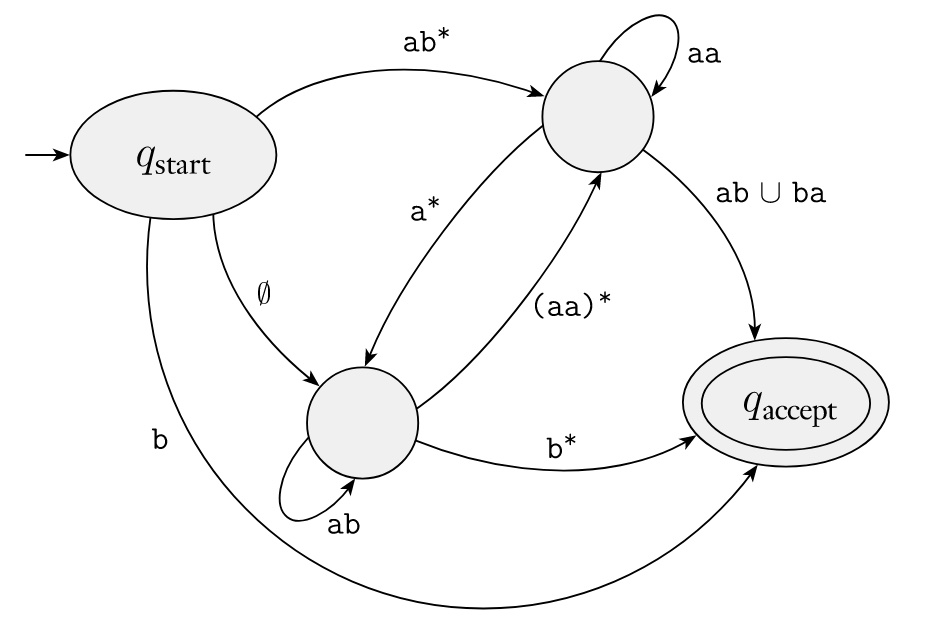
\includegraphics[width=0.8\textwidth]{f1.61.jpg}
\end{eg}

Now we're going to covert GNFA to regular expressions to proof \hyperref[lemma: 2.2]{the Lemma}.

For convenience, we will assume (we can easily modify the machine to achieve):
\begin{itemize}
    \item One accept state, separate from the start state.
    \item One arrow from each state to each state, except
    \begin{itemize}
        \item only exiting the start state
        \item only entering the accept state
    \end{itemize}
\end{itemize}

\begin{lemma}[GNFA -> Regular Expressions]
    Every GNFA \(G\) has an equivalent regular expression R.
\end{lemma}
\begin{proof}
    By induction(recursion) on the number of states \(k\) of G. 

    \hfill\break
    \underline{Basis}(\(k =2\)):G can only looks like:\\ G = ->start --r-->accept\\
    In this case, R = r.

    \hfill\break
    \underline{Induction step(\(k > 2\))}: Assume Lemma true for \(k - 1\) states and prove for \(k\) states \\
    IDEA: Convert \(k\)-state GNFA to equivalent \((k - 1)\)-state GNFA  
    \\
    \begin{enumerate}
        \item First we pick any state \(x\) except the start and accept states.
        \item Remove \(x\).
        \item Repair the damage by recovering all paths that went through x. 
        \item Make the indicated change for each pair of states \(q_i, q_j\).
    \end{enumerate}

    In the following example, this is how we remove a state \(x\):\\
    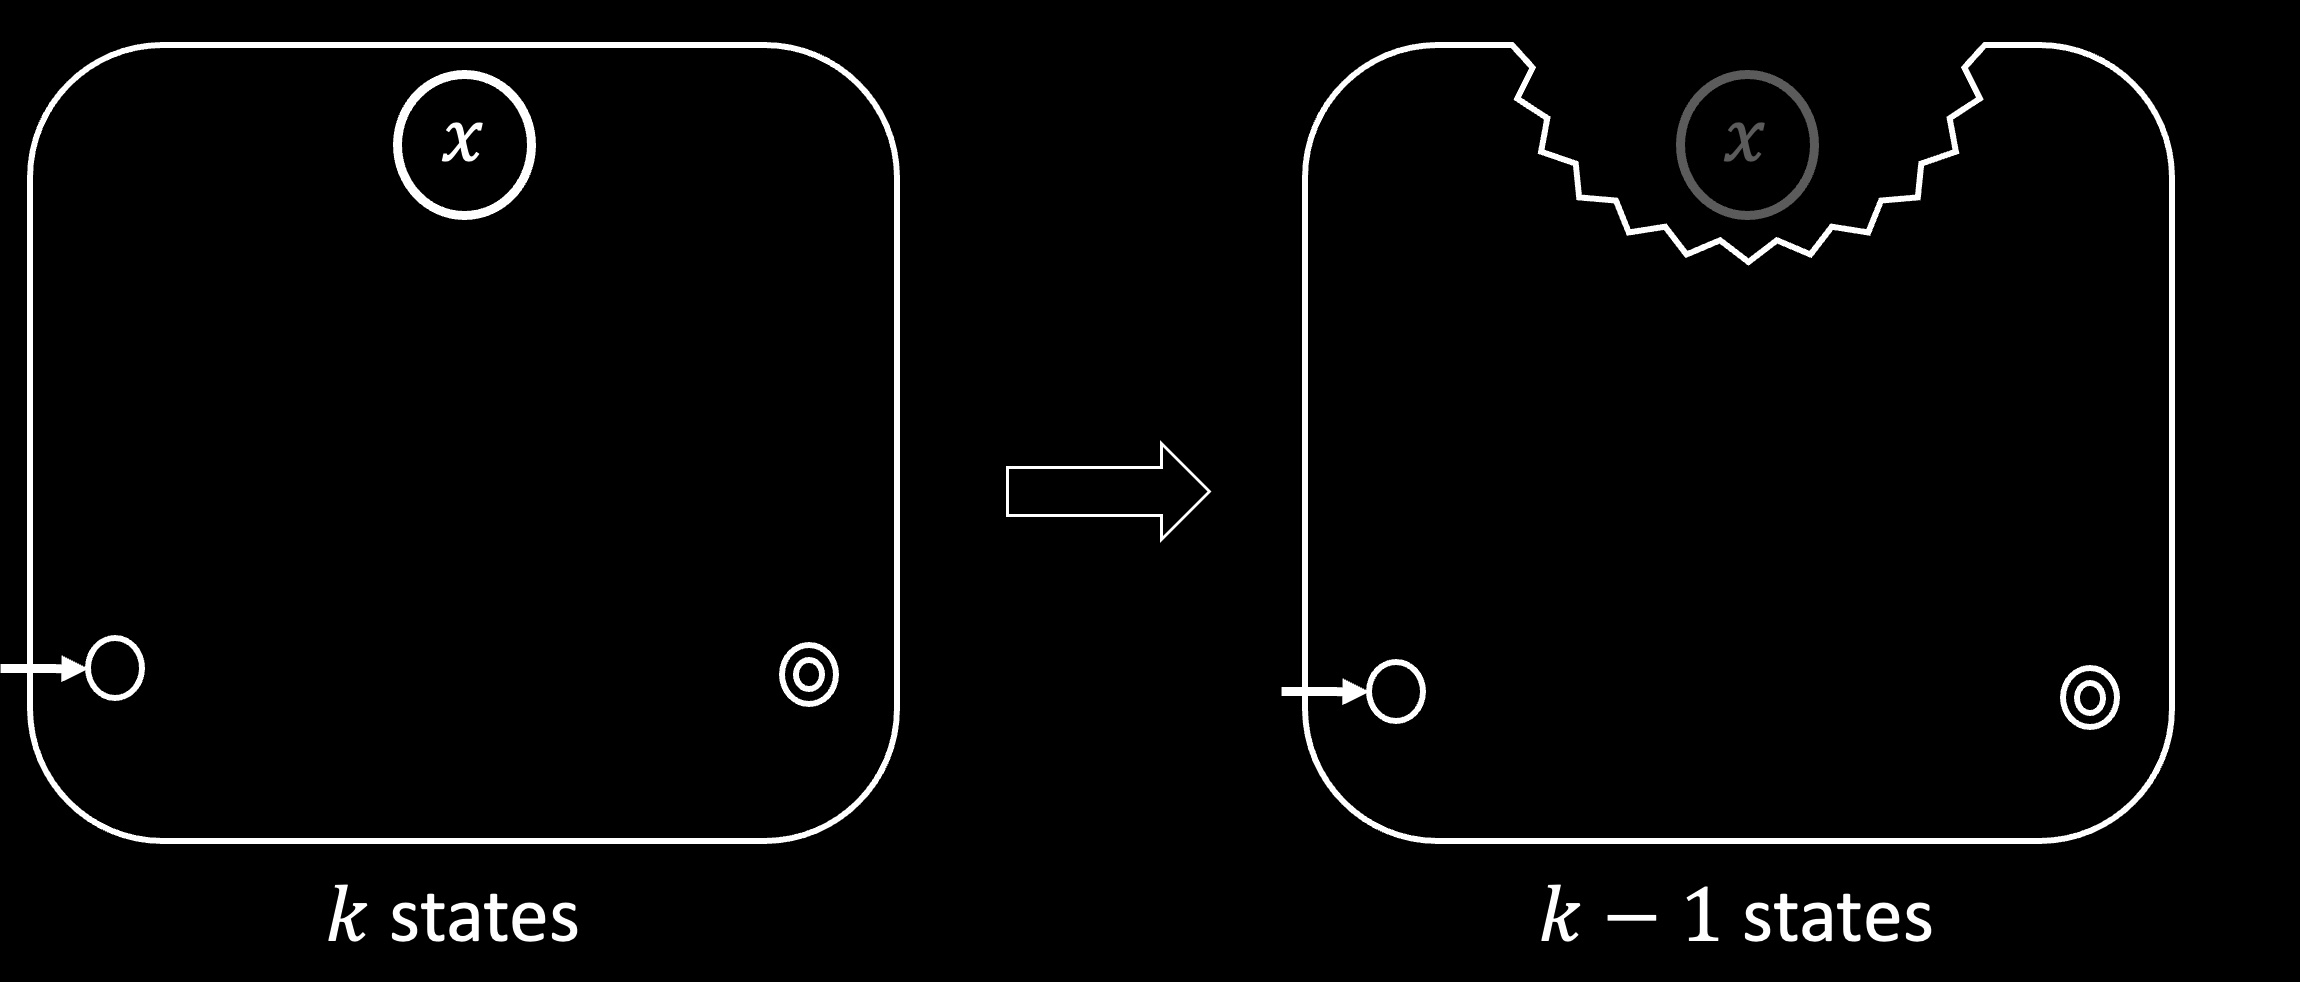
\includegraphics[width=0.8\textwidth]{l3.1.jpg}

    Then we replace the original paths with new paths:\\
    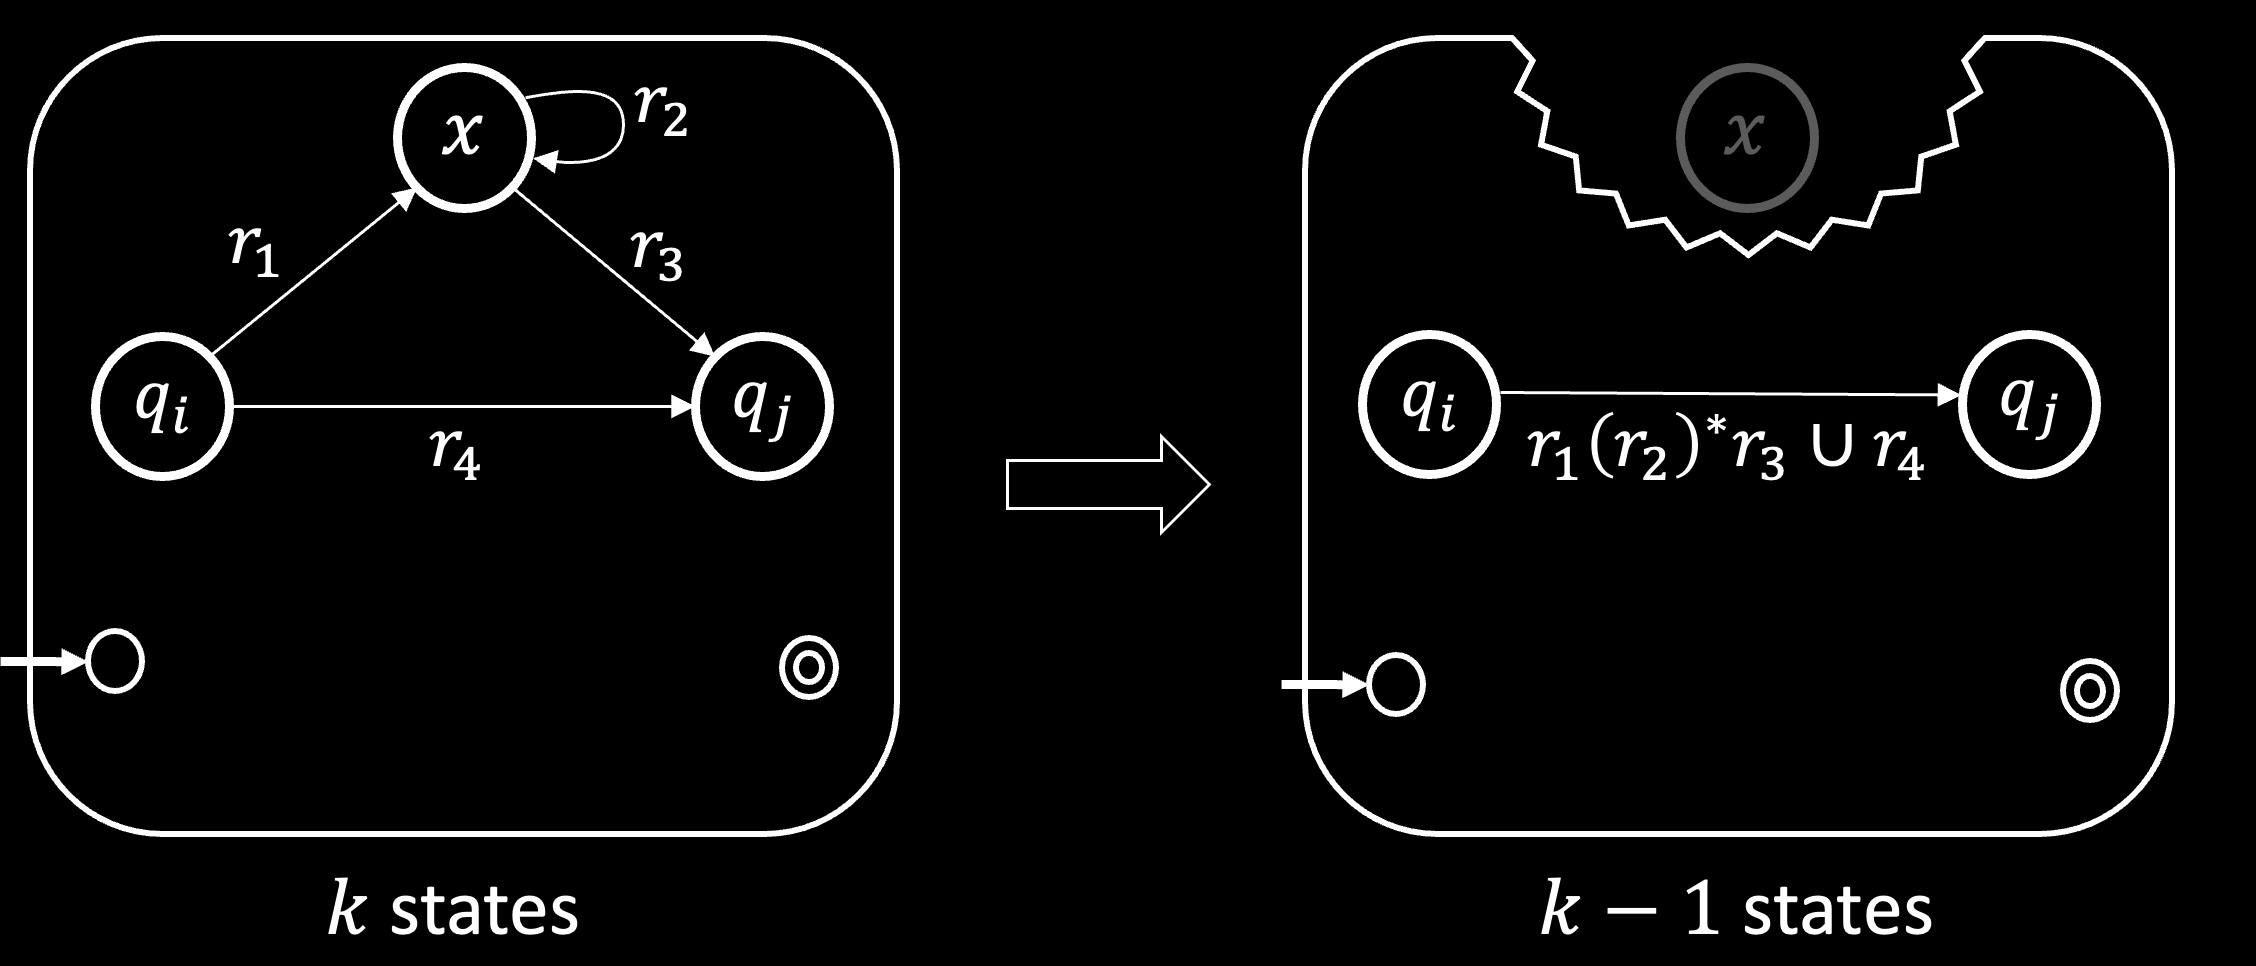
\includegraphics[width=0.8\textwidth]{l3.2.jpg}

    We're already done, because DFAs are a type of GNFAs.
\end{proof}


\section{Non-Regular Languages}
How do we show a language is not regular?
\begin{itemize}
    \item To show a language is regular we give a DFA.
    \item \underline{To show a language is not regular, we must give a proof} (It is not enough to say that you couldn't find a DFA for it, therefore the language is not regular).
\end{itemize}

\begin{eg}
    Here \(\Sigma = \{ 0, 1 \} \) 

    \begin{enumerate}
        \item B has equal numbers of 0 and 1\\
        Intuition: B is not regular because DFAs cannot count unboundedly.
        \item C has equal numbers of \verb|01| and \verb|10| substrings.\\
        \verb|0101| \(\notin\) C \\
        \verb|0110| \(\in\) C\\ 
        Intuition: C is not regular because DFAs cannot count unboundedly. (Wrong! Actually, C is regular!)
    \end{enumerate}

    Moral: You need a proof.
\end{eg}


\section{Pumping Lemma}
Pumping lemma is the method for proving non-regularity.

\begin{lemma}[Pumping Lemma]
    For every regular language A, there's a number \(p\) (the "pumping length") such that  
    if \(s \in A\) and \(|s| \geq p\) then \(s = xyz\) where 
    \begin{enumerate}
        \item \(xy^iz \in A\) for all \(i \geq 0\) \quad \(y^i = yy\cdots y\)(i number of y)
        \item \(y \neq \epsilon\)
        \item \(|xy| \leq p\)     
    \end{enumerate}
    \begin{remark}
        \(|s|\) means the length of the string \verb|s|. 
    \end{remark}
    \hfill \break
    Informally: \(A\) is regular -> every long string in A can be pumped and the result stays in \(A\).  
\end{lemma}
\begin{proof}
    Let DFA \(M\) recognize \(A\). Let \(p\) be the number of states in \(M\). Pick \(s \in A\) where \(|s| \geq p\).      

    When you have a too long string, you inevitably have to revisit the same state again and again, forming the struct as following:

    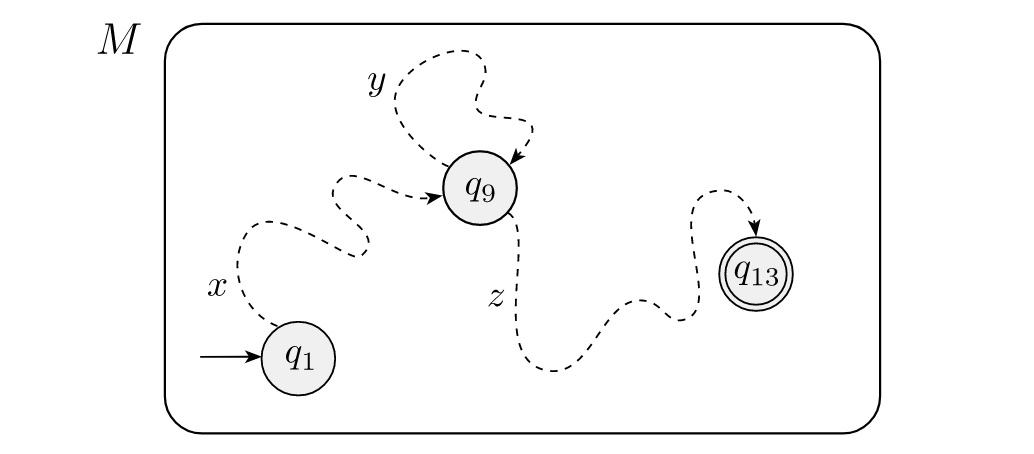
\includegraphics[width=0.8\textwidth]{f1.72.jpg}

    This is also known as The Pigeonhole Principle.
\end{proof}

\begin{eg}[Prove Non-regularity]
    Let \(D = \{ 0^k1^k | k \geq 0 \} \) 
\end{eg}
\begin{proof}
    Show: D is not regular

    Proof by Contradiction:

    Assume that D is regular, applying pumping lemma, let \(s = 0^p1^p \in D\). 

    Pumping lemma says that can divide \(s = xyz\) satisfying the 3 conditions.

    But \(xyyz\) has excess 0s and thus \(xyyz \notin D\) contradicting the pumping lemma.  
\end{proof}

\begin{eg}
    Let \(F = \{ ww| w \in \Sigma^* \} \), Say \(\Sigma^* = \{ 0, 1 \} \)  
\end{eg}
\begin{proof}
    Assume F is regular.\\
    Try \(s = 0^p10^p1 \in F\), show cannot be pumped \(s = xyz\) satisfying the 3 conditions.  
\end{proof}

Variant: Combine closure properties with the pumping lemma.

\begin{eg}
    Let \(B = \{ w | w \)  has equal number of 0s and 1s\}.
\end{eg}
\begin{proof}
    Assume that B is regular.

    We know that \(0^*1^*\) is regular so  \(B \cap 0^*1^*\) is regular (closure under intersection). 

    But \(D = B \cap 0^*1^*\) and we already showed \(D\) is not regular. Contradiction!
\end{proof}


\section{Context Free Grammars}

It is a stronger computation model.


